\documentclass{beamer}
\usetheme{Boadilla}
\usepackage{essay-def}
\usepackage{bm}
\usepackage{amsfonts}
\usepackage{amssymb}
\usepackage{amsmath}
\usepackage{amsthm}
\usepackage{comment}
\usepackage{geometry}
\geometry{left=1cm,right=1cm}
    \title[Stability]{Stability Analysis of Chaotic System}
\author[J. Zhao]{Jiaxi Zhao}
\date{6th July, 2023}
\begin{document}
\par \setlength{\parindent}{2em}

\begin{frame}
\titlepage

\end{frame}


\begin{frame}{Sampling}
	\begin{itemize}
		\item Ergodic \& Chaotic
		\item Lyapunov exponent
		\item Linear Stability Analysis (LSA)
		\item Adjoint method
	\end{itemize}
\end{frame}


\begin{frame}{Maximum Likelihood Principle}
	In classical parametric statistics, suppose one has a statistical model $p(\mfx; \theta)$ and a set of data samples $\mfx_1, \mfx_2, \cdots, \mfx_N$, the maximum likelihood principle provide us with a natural estimator given by:
	\bequn
		\wht\theta = \arg\max_{\theta} \log \prod_{i = 1}^N p(\mfx_i; \theta).
	\eequn
	It is well-known that this estimator can also be viewed as the minimizer of the KL-divergence between the empirical measure and $p(\mfx; \theta)$.
\end{frame}


\begin{frame}{Real World Distribution}
	How about real world distribution? i.e. distribution of all the images, distribution of all the texts. How can we model these distributions and do sampling from them?
	\begin{itemize}
		\item 1. Classical non-parametric approach, e.g. mixture Gaussian model.
		\item 2. Bayesian inference, e.g. variational inference.
		\item 3. Generative adversarial network (GAN), energy-based method (Langevin dynamics), etc.
	\end{itemize}
\end{frame}


\begin{frame}{ELBO and Variational Inference}
	In order to estimate the unknown likelihood function $p(\mfx)$, we introduce ``Evidence lower bound'' (ELBO)
	\bequn
		\log p(\mfx) \geq \mbE_{q_{\phi}(\mfz|\mfx)}\lb \log \frac{p(\mfx, \mfz)}{q_{\phi}(\mfz|\mfx)} \rb
	\eequn
	Here $\phi$ may be any statistical models, either parametric or non-parametric. 
\end{frame}


\begin{frame}{ELBO}
	To prove this, one has
	\bequn
		\begin{aligned}
		\log p(\mfx)  = & \ \mbE_{q_{\phi}(\mfz|\mfx)}\lb \log p(\mfx) \rb  			\\
		= & \ \mbE_{q_{\phi}(\mfz|\mfx)}\lb \log \frac{p(\mfx, \mfz)q_{\phi}(\mfz|\mfx)}{p(\mfz|\mfx)q_{\phi}(\mfz|\mfx)} \rb  			\\
		= & \ \mbE_{q_{\phi}(\mfz|\mfx)}\lb \log \frac{p(\mfx, \mfz)}{q_{\phi}(\mfz|\mfx)} \rb + \mbE_{q_{\phi}(\mfz|\mfx)}\lb \log \frac{q_{\phi}(\mfz|\mfx)}{p(\mfz|\mfx)} \rb  			\\
		\geq & \ \mbE_{q_{\phi}(\mfz|\mfx)}\lb \log \frac{p(\mfx, \mfz)}{q_{\phi}(\mfz|\mfx)} \rb, 			\\
		\end{aligned}
	\eequn
	where the last inequality is based on the observation that $\mbE_{q_{\phi}(\mfz|\mfx)}\lb \log \frac{q_{\phi}(\mfz|\mfx)}{q_{\phi}(\mfz|\mfx)} \rb = D_{\KL}(q_{\phi}(\mfz|\mfx)||p(\mfz|\mfx))$.
\end{frame}


\begin{frame}{First generative model: Variational Autoencoder}
	Based on the simple idea of ELBO, one can introduce our first generative model in this series, i.e. variational autoencoder:
	\bequn
		\begin{aligned}
			\mbE_{q_{\phi}(\mfz|\mfx)}\lb \log \frac{p(\mfx, \mfz)}{q_{\phi}(\mfz|\mfx)} \rb = & \ 
			\mbE_{q_{\phi}(\mfz|\mfx)}\lb \log \frac{p_{\theta}(\mfx| \mfz)p(\mfz)}{q_{\phi}(\mfz|\mfx)} \rb  \\
			= & \ \mbE_{q_{\phi}(\mfz|\mfx)}\lb \log p_{\theta}(\mfx| \mfz) \rb - D_{\KL}(q_{\phi}(\mfz|\mfx)||p(\mfz)).  \\
		\end{aligned}
	\eequn
	Why such a structure is called autoencoder? Encoder: $q_{\phi}(\mfz|\mfx)$, decoder: $p_{\theta}(\mfx| \mfz)$.
	\begin{figure}[H]
          \centering
          \centerline{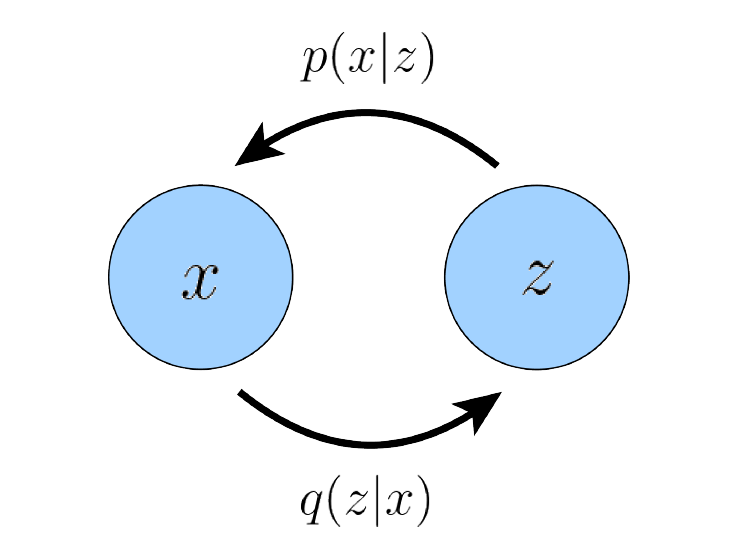
\includegraphics[width=0.3\linewidth]{fig/VAE1.png}}
          \caption{An illustration of VAE\footnotemark}
        \end{figure}
        \footnotetext{Understanding Diffusion Models: A Unified Perspective, Calvin Luo}
\end{frame}


\begin{frame}{VAE}
	The remaining question is: how do we estimate the expectation of ELBO which is divided into two parts?
	 We will pose following ansatz on the form of encoder $q_{\phi}(\mfz|\mfx)$ and prior $p(\mfz)$:
	\bequn
		\begin{aligned}
			q_{\phi}(\mfz|\mfx) & = \mcN(\mfz; \mu_{\phi}(\mfx), \sigma_{\phi}^2(\mfx)\mfI), 			\\
			p(\mfz) & = \mcN(\mfz; \mathbf{0}, \mfI).
		\end{aligned}
	\eequn
	This will reduce $D_{\KL}$ term to an analytic form and we will calculate the first term via Monte Carlo sampling, i.e.
	\bequn
		\arg\max_{\phi, \theta} \sum_{i=1}^l \log p_{\theta}(\mfx| \mfz^{(l)}) - D_{\KL}(q_{\phi}(\mfz|\mfx)||p(\mfz)),
	\eequn
	where $\mfz^{(l)}$ is sampling from $\mcN(\mfz; \mu_{\phi}(\mfx), \sigma_{\phi}^2(\mfx)\mfI)$.
\end{frame}


\begin{frame}{VAE}
	One more question appears: How do we do auto-differentiation in gradient-based optimization?
	
	Here comes the reparameterization trick, by using following computational graph:
	\bequn
		\mfz = \mu_{\phi}(\mfx) + \sigma_{\phi}(\mfx) \odot \epsilon, \quad \epsilon\sim \mcN(\mathbf{0}, \mfI).
	\eequn
	Parameters in $\phi$ is included in the calculation of loss function, therefore auto-differentiation becomes possible.
\end{frame}


\begin{frame}{Second generative model: Hierarchical Variational Autoencoder}
\bequn
	\begin{aligned}
	p(\mfx, \mfz_{1:T}) & = p(\mfz_T)p(\mfx|\mfz_1)\prod_{t=2}^T p(\mfz_{t-1}|\mfz_t), 		\\
	q_{\phi}(\mfz_{1:T}|\mfx) & = q_{\phi}(\mfz_1|\mfx) \prod_{t=2}^T q_{\phi}(\mfz_{t}|\mfz_{t-1}) .
	\end{aligned}
\eequn
\begin{figure}[H]
          \centering
          \centerline{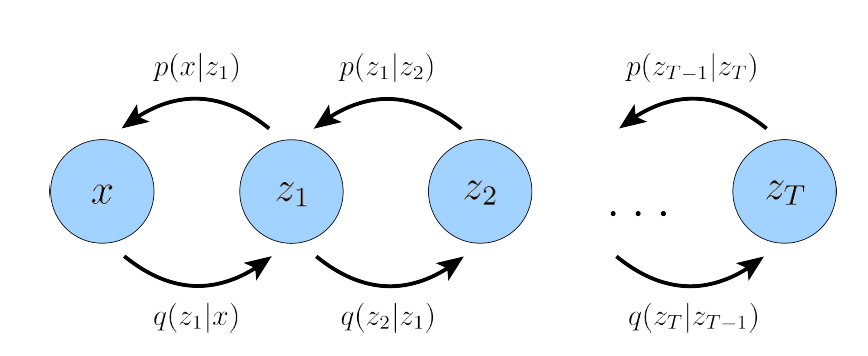
\includegraphics[width=0.6\linewidth]{fig/HVAE.png}}
          \caption{A Markovian Hierarchical Variational Autoencoder\footnotemark with T hierarchical latents. The generative process is modeled as a Markov chain, where each latent $\mfz_t$ is generated only from the previous latent $\mfz_{t+1}$.}
        \end{figure}
        \footnotetext{Understanding Diffusion Models: A Unified Perspective, Calvin Luo}
\end{frame}


\begin{frame}{Third generative model: Variational Diffusion Model}
	We can finally go to the description of the variational diffusion model, one can think of VDM as a MHVAE with following requirement:
	\begin{itemize}
		\item 1. The latent dimension is exactly equal to the data dimension, we use $\mfx_{1:T}$ to denote latent variables.
		\item 2. The structure of the latent encoder at each time step is pre-defined as a linear Gaussian model, i.e. $q_{\phi}(\mfx_t|\mfx_{t-1}) = q(\mfx_t|\mfx_{t-1}) = \mcN(\mfx_t; \sqrt{\alpha_t}\mfx_{t-1}, (1-\alpha_t)\mfI)$.
		\item 3. $p(\mfx_T) \sim \mcN(\mathbf{0}, \mfI).$
	\end{itemize}
	\begin{figure}[H]
          \centering
          \centerline{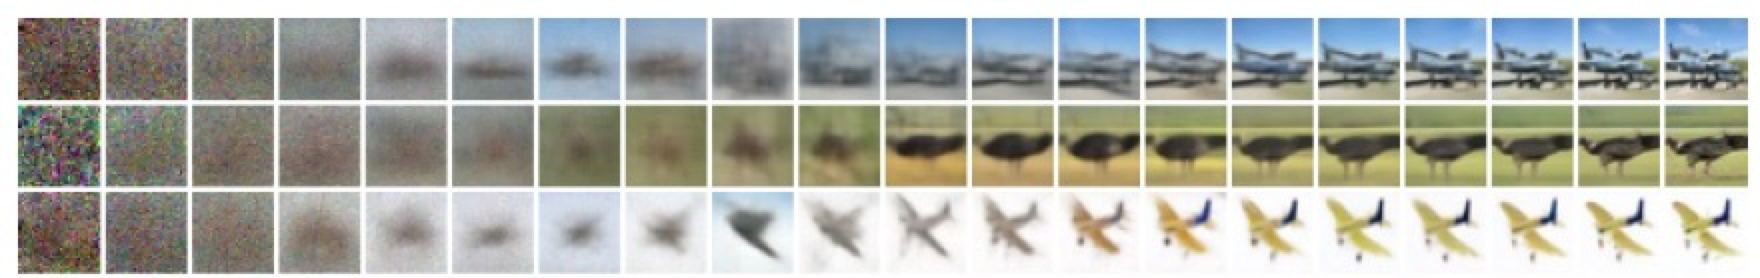
\includegraphics[width=\linewidth]{fig/VDM.png}}
          \caption{Sampling along the trajectories of a diffusion model\footnotemark.}
        \end{figure}
        \footnotetext{Denoising Diffusion Probabilistic Models, Jonathan Ho et. al.}
\end{frame}


\begin{frame}{VDM}
	Based on this framework, one can calculate the ELBO as follows:
	\bequn
		\begin{aligned}
			\log p(\mfx) \geq & \ \mbE_{q(\mfx_{1:T}|\mfx_0)}\lb \log \frac{p(\mfx_{0:T})}{q(\mfx_{1:T}|\mfx_0)} \rb 				\\
			= & \ \mbE\lb \log \frac{p(\mfx_{T})p_{\theta}(\mfx_0|\mfx_1)}{q(\mfx_{T}|\mfx_{T-1})} \rb + \mbE\lb \log \prod_{t=1}^{T-1}\frac{p_{\theta}(\mfx_t|\mfx_{t+1})}{q(\mfx_{t}|\mfx_{t-1})} \rb 		\\
			= & \ \mbE_{q(\mfx_1|\mfx_0)}\lb \log p_{\theta}(\mfx_0|\mfx_1)\rb + \mbE_{q(\mfx_T, \mfx_{T-1}|\mfx_0)}\lb \log \frac{p(\mfx_{T})}{q(\mfx_{T}|\mfx_{T-1})} \rb 		\\
			& \ + \sum_{t = 1}^{T-1}\mbE_{q(\mfx_{t+1}, \mfx_{t-1}, \mfx_t|\mfx_0)}\lb \log \frac{p_{\theta}(\mfx_t|\mfx_{t+1})}{q(\mfx_{t}|\mfx_{t-1})} \rb 		\\
			= & \ \mbE_{q(\mfx_1|\mfx_0)}\lb \log p_{\theta}(\mfx_0|\mfx_1)\rb - \mbE_{q(\mfx_{T-1}|\mfx_0)}D_{\KL}(q(\mfx_{T}|\mfx_{T-1})||p(\mfx_{T})) 		\\
			& \ - \sum_{t = 1}^{T-1}\mbE_{q(\mfx_{t+1}, \mfx_{t-1}|\mfx_0)} D_{\KL}(q(\mfx_{t}|\mfx_{t-1})||p_{\theta}(\mfx_{t}|\mfx_{t+1})).
		\end{aligned}
	\eequn
\end{frame}


\begin{frame}{VDM}
	Let us have a brief interpretation of the terms in this expansion:
	\begin{itemize}
		\item 1. $\mbE_{q(\mfx_1|\mfx_0)}\lb \log p_{\theta}(\mfx_0|\mfx_1)\rb$: reconstruction term, same as VAE.
		\item 2. $\mbE_{q(\mfx_{T-1}|\mfx_0)}D_{\KL}(q(\mfx_{T}|\mfx_{T-1})||p(\mfx_{T}))$: prior matching term, no trainable parameters.
		\item 3. $\sum_{t = 1}^{T-1}\mbE_{q(\mfx_{t+1}, \mfx_{t-1}|\mfx_0)} D_{\KL}(q(\mfx_{t}|\mfx_{t-1})||p_{\theta}(\mfx_{t}|\mfx_{t+1}))$: consistency term, related to reversibility.
	\end{itemize}
\end{frame}


\begin{frame}{VDM}
	Using Bayesian rule, one can rearrange the term to simplify the expectation we are dealt with:
	\bequn
		\begin{aligned}
			\log p(\mfx) = & \ \mbE_{q(\mfx_1|\mfx_0)}\lb \log p_{\theta}(\mfx_0|\mfx_1)\rb - D_{\KL}(q(\mfx_{T}|\mfx_{0})||p(\mfx_{T})) 		\\
			& \ - \sum_{t = 1}^{T-1}\mbE_{q(\mfx_{t+1}, \mfx_{0})} D_{\KL}(q(\mfx_{t}|\mfx_{t+1},\mfx_0)||p_{\theta}(\mfx_{t}|\mfx_{t+1})).
		\end{aligned}
	\eequn
	The last term is now called denoising matching term.
\end{frame}


\begin{frame}{VDM}
	Again the practical question is: How to optimize such a complicated objective function? We will significant reduce the calculation by leveraging the Gaussian transition assumption, i.e.
	\bequn
		q(\mfx_{t}|\mfx_{t+1},\mfx_0) = \frac{q(\mfx_t|\mfx_{t-1}, \mfx_0)q(\mfx_{t-1}|\mfx_0)}{q(\mfx_t|\mfx_0)}.
	\eequn
	Hence, it suffices to derive $q(\mfx_t|\mfx_0)$:
	\bequn	
		\begin{aligned}
		\mfx_t = & \ \sqrt{\alpha_t} \mfx_{t-1} + \sqrt{1-\alpha_t} \epsilon_{t-1}		\\
		= & \ \sqrt{\alpha_t} \lp\sqrt{\alpha_{t-1}} \mfx_{t-2} + \sqrt{1-\alpha_{t-1}} \epsilon_{t-2}\rp + \sqrt{1-\alpha_t} \epsilon_{t-1}		\\
		= & \ \sqrt{\alpha_t\alpha_{t-1}}\mfx_{t-2} + \sqrt{1-\alpha_t\alpha_{t-1}}\epsilon.
		\end{aligned}
	\eequn
\end{frame}


\begin{frame}{VDM}
	Based on the previous calculation, one obtains
	\bequn
		q(\mfx_{t}|\mfx_{t+1},\mfx_0) = \mcN\lp \mfx_{t-1}; \frac{\sqrt{\bar{\alpha}_t}(1-\alpha_t)\mfx_0 + \sqrt{\alpha_t}(1-\bar{\alpha}_t)\mfx_t}{1-\bar{\alpha}_t}, \Sigma_q(t) \rp,
	\eequn
	where $\bar{\alpha} = \prod_{t=1}^T\alpha_t, \Sigma_q(t) = \frac{(1-\alpha_t)(1-\bar{\alpha}_t)}{1-\bar{\alpha}_t}\mfI.$ Therefore, it makes sense to set
	\bequn
		\begin{aligned}
			p_{\theta}(\mfx_{t-1}|\mfx_t) = & \ \mcN(\mu_{\theta}(\mfx_t, t), \Sigma_q(t)), 		\\
			\mu_{\theta}(\mfx_t, t) = & \ \frac{\sqrt{\bar{\alpha}_t}(1-\alpha_t)\mfx_0 + \sqrt{\alpha_t}(1-\bar{\alpha}_t)\mfx_{\theta}(\mfx_t, t)}{1-\bar{\alpha}_t}.
		\end{aligned}
	\eequn
\end{frame}



\begin{frame}{Advantages of Diffusion models}
	Diffusion models have following advantages:
	\begin{itemize}
		\item 1. Comparing to GAN, it is more robust to mode collapse, successfully apply to multimodal distribution. Some combination with sampling technique in determinantal point process is also transplanted to diffusion models.
		\item 2. It processes solid theoretic foundation and shares lots of connection with energy-based sampler, score-matching sampler.
	\end{itemize}

\end{frame}


\begin{frame}{Disadvantages of Diffusion models}
	On the other hand, several disadvantages remain
	\begin{itemize}
		\item 1. Since one requires the prior for $\mfx_T$ to be standard Gaussian, the time horizon is usually taken to be a large number, which makes the training and sampling much more expansive than other methods such as GAN.
		\item 2. The accuracy of the sampling is not comparable to SOTA, i.e. various modification of GAN.
		\item 3. Currently, there is no satisfying theory on choosing the diffusion norse parameters $\alpha_t$.
	\end{itemize}

\end{frame}


\begin{frame}{Reference}
	\begin{itemize}
		\item 1. Luo, Calvin. "Understanding diffusion models: A unified perspective." arXiv preprint arXiv:2208.11970 (2022).
		\item 2. Ho, Jonathan, Ajay Jain, and Pieter Abbeel. "Denoising diffusion probabilistic models." Advances in Neural Information Processing Systems 33 (2020): 6840-6851.
		\item 3. Tutorial on Denoising Diffusion-based Generative Modeling: Foundations and Applications: https://www.youtube.com/watch?v=cS6JQpEY9cs\&t=1948s
	\end{itemize}

\end{frame}







\end{document}